\documentclass{article}
\usepackage{times}
\usepackage{a4wide}
\usepackage{latexsym}
\usepackage{mathrsfs}
\usepackage{amsmath}
\usepackage{amssymb}
\usepackage{amsthm}
\usepackage{ifthen}
\usepackage{stmaryrd}
\usepackage{algorithm}
%\usepackage{algorithmic}
\usepackage{algpseudocode}
\usepackage{graphics}
\usepackage{epsfig}
%\usepackage{ramacros}

\addtolength{\textwidth}{20mm}
\addtolength{\oddsidemargin}{-10mm}
\addtolength{\textheight}{18mm}
\addtolength{\topmargin}{-9mm}

\newcounter{exercise}
\setcounter{exercise}{0}
\newcommand{\exercise}{
        \addtocounter{exercise}{1}
        \vspace{0.2in}
        \noindent
        {\bf \theexercise .}
        }

\newcommand{\REMARK}[1]{}


\newcommand{\NEWPART}{\vspace{.1in}
              \noindent}

\newcommand{\<}{
    \langle}

\renewcommand{\>}{
    \rangle}

\newcommand{\ceil}[1]{\left\lceil #1 \right\rceil}

\pagestyle{plain} \pagenumbering{arabic}

\title{{\bf Assignment 3} \\ {\large ID: 120037910002 } {\large Name: Xingguo Jia } {\large Email: jiaxg1998@sjtu.edu.cn}}

\author{}
\date{}

\begin{document}
\maketitle

%{\large \noindent
%\begin{tabular}{lcl}
%{Jan 17 2007}.
%\end{tabular}
%}

{\large





\begin{exercise}
Prove or disprove the following statement. If all capacities in a network are distinct,
 then there exists a unique flow function that gives the maximum flow.
\end{exercise}

\textbf{Disprove:}

\begin{itemize}
    \item See Figure \ref{a}, each edge has a distinct capacity, but we have two flow functions $f_1,f_2$ that both give the maximum flow, where

    \centering $f_1(s,A)=f_1(A,B)=f_1(B,t)=2$ and $f_1(e)=0$ for other edges,
    
    \centering $f_2(s,C)=f_2(C,B)=f_2(B,t)=2$ and $f_2(e)=0$ for other edges.
\end{itemize}

\begin{figure}[!htp]
    \centering
    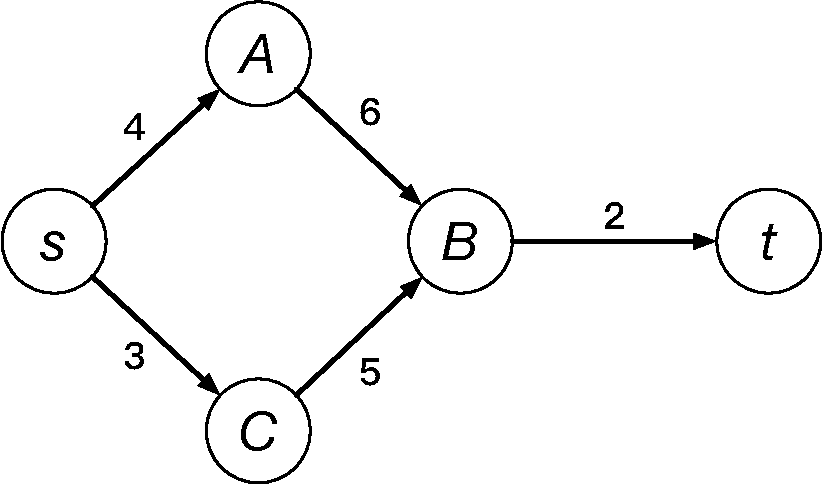
\includegraphics[width=0.4\textwidth]{img/a.pdf}
    \caption{Graph with two maximum flow functions}
    \label{a}
\end{figure}

\newpage


\begin{exercise}
An edge of a flow network is called \textbf{critical} if decreasing the capacity of this edge results in a decrease in the maximum flow value. Present an efficient algorithm that, given an $s$-$t$ network $G$ finds any critical edge in a network(assuming one exists).
\end{exercise}

\textbf{Solution:}
\begin{itemize}
    \item If an edge is not filled to capacity in the maximum flow, then decreasing its capacity will not result in a decrease in the maximum flow value. Thus, a \textbf{critical} edge must be full edge in the maximum flow of the graph.
    \item We run Ford-Fulkerson algorithm on the graph $G$ and get residual graph $G_f$. For each full edge $(u,v)$, we do DFS from $u$ to $v$ on $G_f$. If there is a path $P$ from $u$ to $v$, then we can decrease the capacity of $(u,v)$ and increase the same amount of flow on $P$ so the maximum flow value does not change, thus $(u,v)$ is not critical path.The following algorithm gives any critical edge:
    \begin{algorithm}[htb]
        \caption{Find any critical edge}
        \begin{algorithmic}[1]
            \State{$G_f\leftarrow $Ford-Fulkerson$(G)$}
            \For{$(u_0,v_0)\in \{(u,v)|(u,v)\in G,(u,v)\notin G_f, (v,u)\in G_f\}$}
                \State DFS$(G_f,u_0)$
                \If {$u_0$ has no path to $v_0$}
                \State
                    \Return $(u_0,v_0)$
                \EndIf
            \EndFor
        \end{algorithmic}
    \end{algorithm}
\end{itemize}
\newpage


\begin{exercise}
Let $G=(V,E)$ be an undirected weighted graph with two distinguished vertices $s,t\in V$. Give an efficient algorithm to find a minimum weight cut that separates $s$ from $t$.
\end{exercise}

\textbf{Solution:}
\begin{itemize}
    \item We transform $G$ to directed graph $G'=(V,E')$. For all edge $(s,u)\in E$, we have $(s,u)\in E'$. For all edge $(v,t)\in E$, we have $(v,t)\in E'$. For all edge $(u,v)\in E$ where $u,v\notin\{s,t\}$, we have $(u,v),(v,u)\in E'$. 
    \item We run Ford-Fulkerson algorithm on $G'$, and we can get a minimum weight cut that separates $s$ from $t$.
\end{itemize}
\newpage


\begin{exercise}
You are given a matrix with fractional elements between $0$ and $1$. The sum of all numbers in each row and in each column is integer. Prove that we can always round each element to $0$ or $1$ so that the sum of each row and each column remains unchanged and design a polynomial time algorithm to find such a rounding result.
\end{exercise}

\textbf{Solution:}
\begin{itemize}
    \item For row $i,1\leq i\leq n$ of the matrix, we construct a row vertex $R_i$. For column $j,1\leq j\leq n$ of the matrix, we construct a column vertex $C_j$. Also construct a source $s$ and a sink $t$.
    \item We construct a directed edge $(s,R_i)$ with capacity of sum row $i$ and a directed edge $(C_j,t)$ with capacity of sum column $j$. For each $R_i$ and $C_j$, we have a directed edge $(R_i,C_j)$ with capacity $1$, and its flow $0\leq f(i,j)\leq 1$ represents the element $M(i,j)$ in the matrix.
    \item Then $f$ is a maximum flow of the constructed graph, where the maximum flow value is the sum of  $M$.
    \item We run Ford-Fulkerson algorithm on the constructed graph, and since all edges have integer capacity, we could find the maximum flow where $f^*(i,j)\in \{0,1\}$ in \textbf{polynomial} time, and thus we find a matrix $M^*(i,j)=f^*(i,j)$ with all elements $\in \{0,1\}$.
\end{itemize}
\newpage


\begin{exercise}
Suppose that, in addition to edge capacities, a flow network has \textbf{vertex capacities}.
That is each vertex has a limit on how much flow can pass though. Show how to transform a flow network $G=(V,E)$ with vertex capacities into an equivalent flow network $G'=(V',E')$ without vertex capacities, such that a maximum flow in $G'$ has the same value as a maximum flow in $G$. How many vertices and edges does $G'$ have?
\end{exercise}

\textbf{Solution:}
\begin{itemize}
    \item For each $v\in V$, we have $v_{in},v_{out}\in V'$ and $(v_{in},v_{out})\in E'$. For each in edge $(a,v)\in E$, we have $(a,v_{in})\in E'$, and for each out edge $(v,b)\in E$, we have $(v_{out},b)\in E'$.
    \item Let $cap(v_{in},v_{out})=cap(v)$. Thus, the in/out flow of $v$ never exceeds $cap(v)$. In this way, the maximum flow of $G'=(V',E')$ can be transformed into the maximum flow of $G$ with \textbf{vertex capacities}.
    \item We have $|V'|=2|V|$ and $|E'|=|E|+|V|$.
\end{itemize}
\newpage



\begin{exercise}
Consider a bipartite graph $G=(X\cup Y,E)$ with parts $X$ and $Y$. Each part contains $2k$ vertices (i.e. $|X|=|Y|=2k$). Suppose that $deg(u)\geq k$ for every $u\in X\cup Y$. Prove that $G$ has a perfect matching.
\end{exercise}

\textbf{Solution:}
\begin{itemize}
    \item For subset $S\subseteq L$ with $1\leq|S|\leq k$, we have $N(S)\geq deg(u)\geq k\geq |S|$, where $u\in S$.
    \item For subset $S\subseteq L$ with $k<|S|\leq 2k$, consider any vertex $v \in Y\setminus N(S)$. Thus $N(v)\cap S=\varnothing$. Since $deg(v)\geq k$, $|N(v)|\geq k$. Then 
    \begin{displaymath} 
        2k=|Y|\geq |S|+|N(v)|>k+k=2k
    \end{displaymath}
    \item which is a contradiction. Thus, we have $N(S)=Y$, and $|N(S)|=|Y|=2k\geq |S|$.
    \item In conclusion, for all $S\subseteq L$, $|N(S)|\geq |S|$. According to Hall's Marriage Theorem, $G$ has a perfect matching.
\end{itemize}
\newpage



\begin{exercise}
You are designing a experiment in which you want to measure certain properties $p_1,\ldots ,p_n$ of a yeast culture. You have a set of tools $t_1,\ldots ,t_m$ that can each measure a subset $S_i$ of the properties. For example, tool $t_i$ measures $S_i$ may equal $\{p_7,p_8\}$. To be sure that your results are not due to noise or other artifact, you must measure every property at least $k$ times using $k$ different tools.
\begin{itemize}
\item Give a polynomial-time algorithm that decides whether the tools you have are sufficient to measure the desired properties the desired number of times.
\item Suppose each tool $t_i$ comes from manufacturer $M_i$ and we have the additional constraint that the tools to test any property $p_i$ can't all come from the same manufacturer. Give a polynomial-time algorithm to solve this problem.
\end{itemize}
\end{exercise}
\textbf{Solution:}
\begin{itemize}
    \item We reduce the first problem to a maximum flow problem with lower bounds.
    \item We add vertices $p_1,\ldots ,p_n$ and $t_1,\ldots ,t_m$, and if tool $t_j$ can measure property $p_i$, we add a directed edge $(t_i,p_j)$.
    \item Add source $s$ and edges $(s,p_i)$, where $cap(s,p_i)=|S_i|$. Add sink $t$ and edges $(t_j,t)$, where $k\leq cap(t_j,t)\leq m$.
    \item We shift the capacity of $(t_j,t)$ to $[0,m-k]$ and set $d(p_j)=k,d(t)=-nk$. Add sink $s^*$ and $t^*$. For vertices with $d(v)<0$, add edge $(s',v)$ with capacity $-d(v)$. For vertices with $d(v)>0$, add edge $(v,t^*)$ with capacity $d(v)$.
    \item In this flow graph, if we could find a flow of value $nk$, the tools are sufficient to measure the desired properties the desired number of times.
    \newline
    \newline
    \item We reduce the second problem to a maximum flow problem.
    \item We add vertices $p_1,\ldots ,p_n$ and $t_1,\ldots ,t_m$. For each $t_j$, we add $m$ vertices $M_{ij},1\leq i\leq m,1\leq j\leq n$ to represent all $m$ manufacturers, where $M_{i1}=M_{i2}=\cdots M_{in}$.
    \item Add edges $(t_j, M_{ij})$ with capacity $1$ if tool $t_j$ comes from manufacturer $M_{ij}$. Add edges $(M_{ij}, p_j),1\leq j\leq n$ with capacity $k-1$ to avoid using tools that come from all the same manufacturer. Add source and sink $s,t$. Add edges $(s,t_j)$ with $+\infty$ capacity, add edges $(p_i,t)$ with $k$ capacity.
    \item If we could find a maximum flow of value $nk$, the tools are sufficient to measure the desired properties the desired number of times with the additional constraint. We could find this maximum flow with Ford-Fulkerson algorithm, which runs in polynomial time.

\end{itemize}
\newpage



\begin{exercise}
Consider a flow network $G=(V,E)$ with positive edge capacities $\{c(e)\}$. Let $f:E\rightarrow \mathbb{R}_{\geq 0}$ be a maximum flow in $G$, and $G_f$ be the residual graph. Denote by $S$ the set of nodes reachable from $s$ in $G_f$ and by $T$ the set of nodes from which $t$ is reachable in $G_f$.  Prove that $V=S\cup T$ if and only if $G$ has a \textbf{unique} $s$-$t$ minimum cut.
\end{exercise}

\textbf{Solution:}
\begin{itemize}
    \item First, we notice that $S\cap T=\varnothing$, since if a vertex $v\in S$ and $v\in T$, we could go from $s$ through $v$ to $t$ in the residual graph, and increase the maximum flow, which is a contradiction.
    \item $\Rightarrow$: We have $C_1=(S,V\setminus S)$ and $C_2=(T,V\setminus T)$ to be minimum cuts of $G$. Since $V=S\cup T$ and $S\cap T=\varnothing$, we have $C_1=C_2$, which means $s$-$t$ minimum cut of $G$ is unique.
    \item $\Leftarrow$: We prove by contradiction. Suppose $S\cup T\subset V$, and let
    \begin{displaymath}
        X=V\setminus(S\cup T),X\neq \varnothing
    \end{displaymath}
    \item Since $C_1=(S\cup X,T)$ and $C_2=(S,X\cup T)$ are two distinct minimum cut, we have a contradiction.
    
\end{itemize}
\newpage



\end{document}
